\section{Data Lab}

\subsection{Implementation of \texttt{howManyBits(x)}}

The goal of this algorithm is to find the minimum number of bits required to represent the given 32-bit number using two's complement.

My implementation of \code{howManyBits(x)} has the following structure:

\begin{enumerate}
  \item Find the absolute value of \code{x}
  \item Find out how many bits are required to represent that value
  \item Add 1 to the result from step 2 to account for the sign bit
\end{enumerate}

Finding the absolute value of \code{x} lets us simplify the problem instead of handling positive and negative numbers separately. And once we've found the required number of bits to represent the 

Of these steps, step 2 is the crux. To solve this, my algorithm uses a binary search to find the most significant bit in the given number. The algorithm is as follows:

\begin{enumerate}
  \item See if there is a 1 in the first 16 bits of the number. If yes, we need at least 16 bits to represent the number. If no, we need at most 15 bits.
  \item Split the search space in half. If we found a 1, the new search space is the first half, and if not, it is the second half.
  \item Repeat steps 1 and 2 until 5 iterations have been performed.

    For the second iteration, we will be looking at 8 bits instead of 16. For the third iteration, we will be looking at 4 bits instead of 8, and so on.

    We can stop at 5 because the input is 32 bits long and $\log_2(32) = 5$.
\end{enumerate}

This may become more clear by reading the comments embedded in the code below and the example following that.

\subsubsection{Code and comments for \texttt{howManyBits(x)}}

Below is the full implementation of \code{howManyBits(x)} with comments that I handed in for the Data Lab assignment.

\bgroup
\small
\begin{minted}[bgcolor=LightGray]{c}
int howManyBits(int x) {
  // The general idea:
  // - Find the absolute value
  // - How many bits are required to represent that value?
  // - 1 more bit is needed for the sign

  // We find the absolute value of x. However, to avoid overflow issues with
  // -2147483648, we will have to subtract 1 from the absolute value if x is
  // negative - but the result we're looking for will be equally viable since
  // 0 is the most significant bit for positive two's complement numbers.
  int absMask = ~(1 & (x >> 31)) + 1;
  int abs = (~absMask & x) | (absMask & ~x);

  // We can now count how many bits we need to represent the unsigned number.
  // Due to the limited amount of operations we have at our disposal, we can't
  // search the 32 bits linearly - instead we use a binary search.
  //
  // The algorithm is as follows:
  //   1. Take a half-of-the-bits sized chunk out of the number - initially 16
  //      bits because the full number is 32 bits. That is, we will be looking
  //      at these bits first:
  //
  //          00000000 00000000 00000000 00000000
  //          ^^^^^^^^ ^^^^^^^^
  //
  //   2. Use !! to see if the bit chunk is nonzero
  int hasBits1 = !!(abs >> 16);
  //   3. Shift to the left by 4 (because 1 << 4 = 16, which is what we shifted
  //      right by). If there were any bits in the chunk, res1 now holds 16 as
  //      its value, but if no bits were present, its value is 0. If a bit was
  //      in the left half of the 32, we know we need at least 16 bits, so we
  //      hold onto this value for a bit (no pun intended).
  int res1 = hasBits1 << 4;
  //   4. Shift the number right by the amount of bits we know we need so far.
  //      By doing this, we perform the "binary search" aspect of the algorithm.
  //      If there was a bit in the left half, the next iteration will be
  //      looking at the first half of this left half - meaning these:
  //
  //          00000000 00000000 00000000 00000000
  //          ^^^^^^^^
  //
  //      That's thanks to us shifting the number right by 16 and the next
  //      iteration shifting right by 8. However, if no bit was in the left
  //      half, we shift right by 0, and the next iteration shifts right by 8.
  //      Therefore it will be looking in the first half of the right half:
  //
  //          00000000 00000000 00000000 00000000
  //                            ^^^^^^^^
  int abs1 = abs >> res1;
  //   5. Rinse and repeat with smaller and smaller halves until we've found how
  //      many bits we need in each.

  int hasBits2 = !!(abs1 >> 8);
  int res2 = hasBits2 << 3;
  int abs2 = abs1 >> res2;

  int hasBits3 = !!(abs2 >> 4);
  int res3 = hasBits3 << 2;
  int abs3 = abs2 >> res3;

  int hasBits4 = !!(abs3 >> 2);
  int res4 = hasBits4 << 1;
  int abs4 = abs3 >> res4;

  int hasBits5 = !!(abs4 >> 1);
  int res5 = hasBits5;
  int abs5 = abs4 >> res5;

  // 6. Add up all the different "I need at least X bits" results
  int unsignedBitsRequired = res1 + res2 + res3 + res4 + res5 + abs5;

  // And then we just need one more bit to represent signed numbers.
  return unsignedBitsRequired + 1;
}
\end{minted}
\egroup

\subsubsection{Example walkthrough of \texttt{howManyBits(x)}}

On the next page you can see a walkthrough of how the algorithm finds the answer given the input \code{4201337}. The left column will show all operations on and values of the variables at each step of the algorithm, and the right column will contain a description of the step. Grey bits indicate that we are no longer interested in those bits.

\newpage
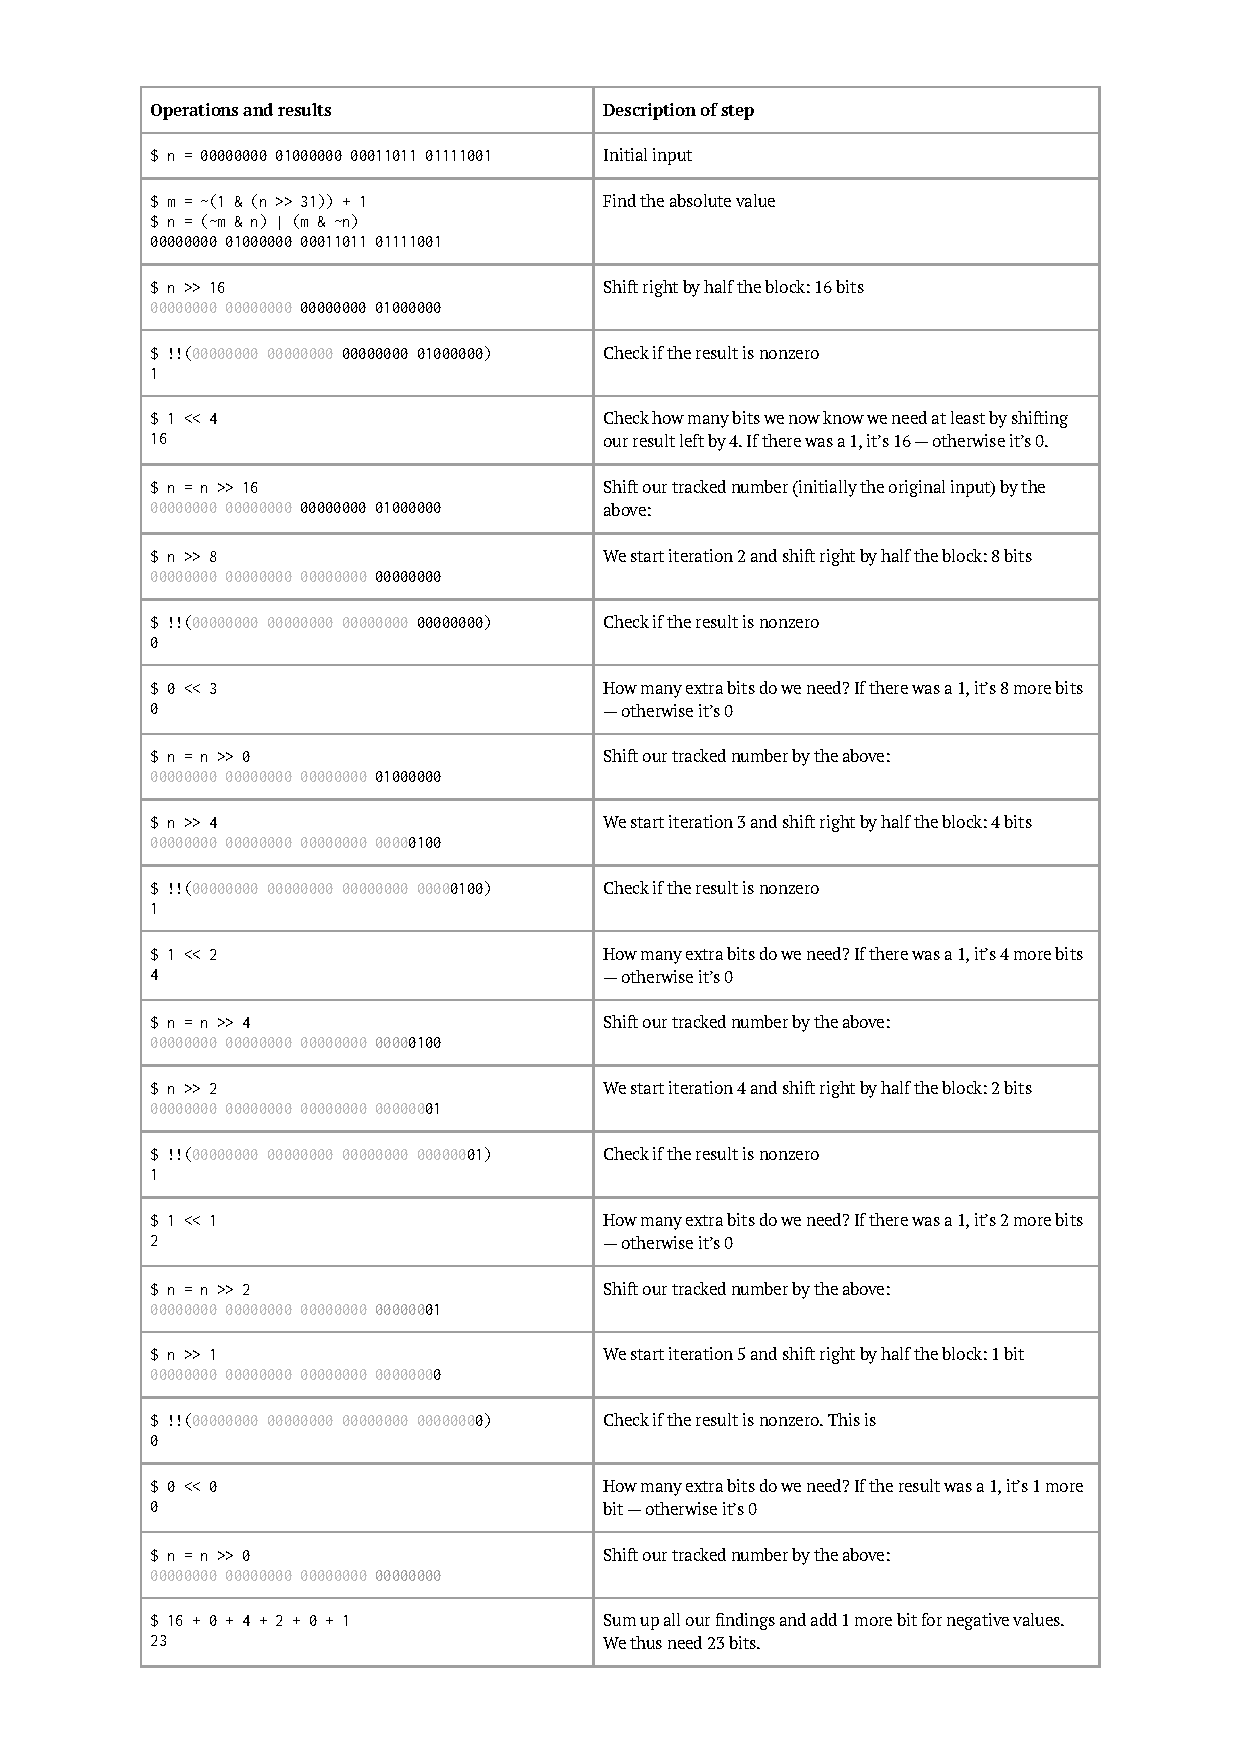
\includepdf[pages=-]{figures/howManyBits-example.pdf}
\newpage
